\chapter{Mathematical Model}

\section{Single Victim Case}
Three Cartesian coordinate frames are defined as \cite{main} and shown in \ref{fig:frames-1victim}:
\begin{enumerate}[label=(\roman*)]
    \item Frame $i$ (inertial): denoted as $F_i = (O_i, x_i, y_i, z_i)$, is the inertial frame with origin $O_i$.
    \item Frame $r$ (receiver ARTVA): denoted as $F_r = (O_r, x_r, y_r, z_r)$, is the body right-hand frame associated with the receiver installed on the drone.
    \item Frame $t$ (transmitter ARTVA): denoted as $F_t = (O_t, x_t, y_t, z_t)$, is the body right-hand frame associated with the transmitter worn by the victim.
\end{enumerate}
For the sake of simplicity, we assume that the body frame of the drone coincides with $F_r$. 
The position of $O_r$ relative to $O_t$ is indicated by the vector $\mathbf{p}_{tr} \in \mathbb{R}^3$, with $\mathbf{p}_{tr} = \mathbf{p}_r - \mathbf{p}_t$, 
while the positions of $O_r$ and $O_t$ relative to $O_i$ are indicated, respectively, by the vectors $\mathbf{p}_r \in \mathbb{R}^3$ and $\mathbf{p}_t \in \mathbb{R}^3$.
We use the apex $i$, $r$ or $t$ on the left of the vector to indicate in which frame the vector is expressed , e.g. ${}^t p$. 
If it is not specified, we assume the inertial frame.
\begin{figure}
    \centering
    \caption{Inertial frames in the single victim case}
    \label{fig:frames-1victim}
    \tdplotsetmaincoords{70}{110}
    \begin{tikzpicture}[tdplot_main_coords]
    \draw[thick,->] (0,0,0) -- (1,0,0) node[anchor=north east]{$y_i$};
    \draw[thick,->] (0,0,0) -- (0,1,0) node[anchor=north west]{$z_i$};
    \draw[thick,->] (0,0,0) -- (0,0,1) node[anchor=south]{$x_i$};
    % Point Pt1
    \coordinate (Pt1) at (5,0,5);
    \draw[->, thick] (0,0,0) -- (Pt1) node[pos=0.5,anchor=east]{${}^i \mathbf{p}_t$};      
    % Point tp
    \coordinate (p1) at (5,5,6);
    \draw[->, thick] (5,0,5) -- (p1) node[pos=0.5,anchor=south]{${}^t \bm{p}_{tr}$};      
    % pr
    \draw[->, thick] (0,0,0) -- (p1) node[pos=0.5,anchor=east]{${}^i \mathbf{p}_r$};

    \node at (p1) [anchor= south west] {$\mathbf{p}$};
    
    \coordinate (Shift) at (5,0,5);
    \tdplotsetrotatedcoordsorigin{(Shift)}
    \draw[thick,tdplot_rotated_coords,->] (0,0,0) --
    (.7,0,0) node[anchor=north]{$y_{t}$};
    \draw[thick,tdplot_rotated_coords,->] (0,0,0) --
    (0,.7,0) node[anchor=north]{$z_{t}$};
    \draw[thick,tdplot_rotated_coords,->] (0,0,0) --
    (0,0,.7) node[anchor=south]{$x_{t}$};
    \coordinate (Shift) at (5,5,6);
    \tdplotsetrotatedcoordsorigin{(Shift)}
    \draw[thick,tdplot_rotated_coords,->] (0,0,0) --
    (.7,0,0) node[anchor=east]{$y_{r}$};
    \draw[thick,tdplot_rotated_coords,->] (0,0,0) --
    (0,.7,0) node[anchor=west]{$z_{r}$};
    \draw[thick,tdplot_rotated_coords,->] (0,0,0) --
    (0,0,.7) node[anchor=south]{$x_{r}$};
    \end{tikzpicture}
\end{figure}
\subsection{Magnitude of Magnetic Field Intensity H}
We have found an expression of $\mathbf{H}$ in spherical coordinates, \ref{eq:H_spheric}, whose magnitude is found as:
\begin{equation}
    \left| \mathbf{H} \right| = \frac{I b^2}{4 \, r^3} \sqrt{ 4 \cos^2 \theta + \sin^2 \theta} = \frac{I b^2}{4 \, r^3} \sqrt{ 3 \cos^2 \theta + 1}
    \label{eq:H_mag_spher}
\end{equation}

\subsubsection{Approximation}
We use the same approximation in \cite{main} in order to remove the non-linearity given by the square root term $\sqrt{ 3 \cos^2 \theta + 1}$. Therefore we approximate:
\[
\frac{1}{\sqrt[3]{ 3 \cos^2 \theta + 1}} \approx \frac{1}{a^2 }\cos^2 \theta + \frac{1}{b^2} \sin^2 \theta
\]
of which the polar plot is shown in Figure \ref{fig:polarplot} when $a$ and $b$ have values 1.291 and 1.028, 
respectively, which minimize the relative mean squared error = 0.123\%.

% with the relative error this are instead the best values
% Best a: 1.284
% Best b: 1.034

Thus, the square root term becomes:
\begin{equation}
    \sqrt{ 3 \cos^2 \theta + 1} \approx \frac{1}{\left(\frac{1}{a^2} \cos^2 \theta + \frac{1}{b^2} \sin^2 \theta\right)^{3/2}}
    \label{eq:approx}
\end{equation}

Using the approximation \eqref{eq:approx} in \eqref{eq:H_mag_spher}:
\begin{equation}
    \left| \mathbf{H} \right| = \frac{I b^2}{4 \, r^3} \left(\frac{1}{a^2} \cos^2 \theta + \frac{1}{b^2} \sin^2 \theta\right)^{2/3}
    \label{eq:H_mag_approx}
\end{equation}

\begin{figure}[h!]
\centering
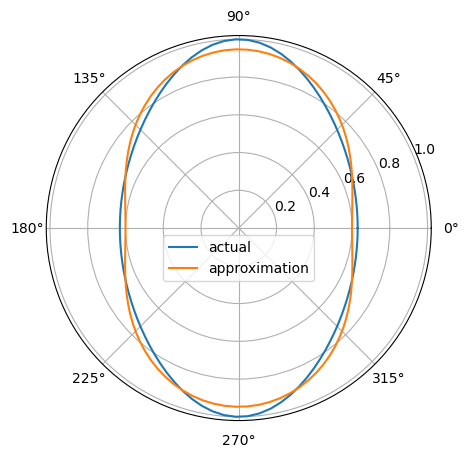
\includegraphics[width=0.5\textwidth]{images/polar_plot.png}
\caption{Polar plot of the actual function $\sqrt{ 3 \cos^2 \theta + 1} $ in blue 
and the approximated one $\frac{1}{a^2 }\cos^2 \theta + \frac{1}{b^2} \sin^2 \theta$ in orange.}
\label{fig:polarplot}
\end{figure}

Now we can express the magnitude using the Cartesian coordinates relative to the frame of the transmitter ARTVA $F_t$. 
If we consider the point ${}^t \mathbf{p}_{tr}$\[
    {}^t \mathbf{p}_{tr} = \begin{pmatrix}
    x \\
    y \\
    z
\end{pmatrix}
\] having these coordinates $(x,y,z)$ in frame $t$, then remembering $r$ from \ref{Conversion from Cartesian to Spherical Coordinates} and $\cos\theta$ from \ref{Conversion from Spherical to Cartesian Coordinates}:
\[
\begin{cases}
r^2 = x^2 + y^2 + z^2 \\
\cos\theta = \frac{x}{r}
\end{cases}
\]

Substituting the expressions for \(r\) and \(\cos\theta\) in \ref{eq:H_mag_approx}:
\[
\left| \mathbf{H} \right| = \frac{I b^2}{4} \frac{1}{(x^2 + y^2 + z^2)^{3}} \left(\frac{1}{a^2} \frac{x^2}{x^2 + y^2 + z^2} + \frac{1}{b^2} \frac{y^2 + z^2}{x^2 + y^2 + z^2}\right)^{2/3}
\]

After simplifications and further calculations, we obtain:
\begin{equation}
    \left| \mathbf{H} \right| = \frac{m}{4 \pi} \left(\frac{(ab)^2}{b^2 x^2 + a^2 (y^2 + z^2)}\right)^{3/2}
    \label{eq:H_mag_cart}
\end{equation}
where we call $I \, \pi \, b^2$ the magnetic moment $m$.
Then, we can define $\eta$ as \cite{main}:
\[ \eta = \left( \frac{m}{4 \pi \left| \mathbf{H} \right|} \right)^{2/3} \cdot \, (ab)^2 = \]
by substituting \ref{eq:H_mag_cart}:
\[
\begin{aligned}
&= \left( \frac{m}{4 \pi \frac{m}{4 \pi} \left(\frac{(ab)^2}{b^2 x^2 + a^2 (y^2 + z^2)}\right)^{3/2}} \right)^{2/3} \cdot (ab)^2 = 
\\
&= \left( \left(\frac{b^2 x^2 + a^2 (y^2 + z^2)}{(ab)^2}\right)^{3/2}\right)^{2/3} \cdot (ab)^2
\end{aligned}
\]

So:
\begin{equation}
    \eta = b^2 x^2 + a^2 (y^2 + z^2)
    \label{eq:eta}
\end{equation}

\subsection{Finding the ARTVA position}
In order to find the victim's position $\mathbf{p}_t$ with respect to the inertial frame $F_i$, we need to use homogeneous transformations \cite{book-robotics}. 
Also from Figure \ref{fig:frames-1victim}, we can express the position of the receiver $\mathbf{p}_r$ in the inertial frame as the sum of the other two vectors:
\[
\begin{aligned}
{}^i \mathbf{p}_r &= {}^i \mathbf{p}_t + {}^t \mathbf{p}_{tr} \\
{}^t \mathbf{p}_{tr} &= R_t^i \,\, {}^i \mathbf{p}_{tr}
\end{aligned}
\]
where $R_t^i$ is the rotation matrix that rotates axis $i$ to $t$ \cite{artva-gazebo}.
\begin{comment}
The matrix $R_t^i$ is the matrix which lets us express the vector in frame $i$ using the coordinates of the vector in frame $t$.Since we are expressing in the columns the coordinates of the axis of $t$ w.r.t using the axis of $i$.
Then if we have the coordinates of point $P$ with respect to frame i $\mathbf{P}$ 
(and if we know the rotation that goes from frame $i$ to frame $t$ (which also means we know the orientation and coordinates of the axis of frame $t$ with respect to those of frame $i$ $(R_t^i$ notation of Soper/this Chapman book), 
we can find the coordinates at point $P$ w.r.t frame i which is $\mathbf{P}$.
Also consider that from frame $i$ after a rotation $R_t^i$ we obtain the same orientation of frame $t$ which is just translated by the $\mathbf{P}_R$ vector.
v1 is  coordinates of the point before the translation but after the rotation, the coordinate of the point wrt the inertial frame  i are v1^i = R p^{i2}
\end{comment}

From which we can find $\mathbf{p}_t$ by multiplying by ${R_t^i}^T$ since ${R_t^i}$ is orthogonal (${R_t^i}^T = {R_t^i}^{-1}$):

\begin{equation}
    {}^t \mathbf{p}_{tr} = {R_t^i}^T (\mathbf{p}_r - \mathbf{p}_t)
    \label{eq:pt}
\end{equation}

In addition, remembering how we defined the coordinates of ${}^t \mathbf{p}_{tr}$, then from linear algebra:
\[
\begin{aligned}
x &= \mathbf{e}_x^T \, {}^t \mathbf{p}_{tr} \\
y &= \mathbf{e}_y^T \, {}^t \mathbf{p}_{tr} \\
x  &= \mathbf{e}_z^T  \, {}^t \mathbf{p}_{tr}
\end{aligned}
\]
also,
\[
x^2 = x \cdot x = \left( \mathbf{e}_x^T \, {}^t \mathbf{p}_{tr} \right)^T \cdot \, \left( \mathbf{e}_x^T \, {}^t \mathbf{p}_{tr} \right)
\]
and the same is valid for the other two coordinates, we will omit the calculations for the other two from now on. 
We can then substitute the expression we found for ${}^t \mathbf{p}_{tr}$ \ref{eq:pt} and apply linear algebra properties of the transpose:
$$(ABC)^T = C^T B^T A^T$$ to calculate the transpose of $\mathbf{e}_x^T {R_t^i}^T (\mathbf{p}_r - \mathbf{p}_t)$:

\[
(\mathbf{e}_x^T {R_t^i}^T (\mathbf{p}_r - \mathbf{p}_t))^T = (\mathbf{p}_r - \mathbf{p}_t)^T {R_t^i} \mathbf{e}_x
\]
The expression for $x^2$ then becomes:
\begin{equation}
    x^2 = \left(\mathbf{p}_r - \mathbf{p}_t\right)^T {R_t^i} \mathbf{e}_x \mathbf{e}_x^T {R_t^i}^T \left(\mathbf{p}_r - \mathbf{p}_t\right)
    \label{eq:x2}
\end{equation}

Furthermore:
\[
\mathbf{e}_x \mathbf{e}_x^T =\begin{pmatrix}
1 \\
0 \\
0
\end{pmatrix}
\begin{pmatrix}
1 & 0 & 0
\end{pmatrix}
 = \text{diag}(1,0,0)
\]
and:
\[
\begin{aligned}
    \mathbf{e}_y \mathbf{e}_y^T &= \text{diag}(0,1,0) \\
    \mathbf{e}_z \mathbf{e}_z^T &= \text{diag}(0,0,1)
\end{aligned}
\]
Lastly we substitute the result found in \ref{eq:x2} in the expression of $\eta$ \ref{eq:eta}:
\[
\begin{aligned}
    \eta &=  \ b^2 \left(\mathbf{p}_r - \mathbf{p}_t\right)^T R_t^i \mathbf{e}_x \mathbf{e}_x^T {R_t^i}^T \left(\mathbf{p}_r - \mathbf{p}_t\right) + \\
    &+ a^2 \left(\mathbf{p}_r - \mathbf{p}_t\right)^T R_t^i \mathbf{e}_y \mathbf{e}_y^T {R_t^i}^T \left(\mathbf{p}_r - \mathbf{p}_t\right) +\\
    &+ a^2 \left(\mathbf{p}_r - \mathbf{p}_t\right)^T R_t^i \mathbf{e}_z \mathbf{e}_z^T {R_t^i}^T \left(\mathbf{p}_r - \mathbf{p}_t\right) =
\end{aligned}
\]
collect common terms,
\[
= \left(\mathbf{p}_r - \mathbf{p}_t\right)^T R_t^i \left( b^2 \mathbf{e}_x \mathbf{e}_x^T + a^2 \mathbf{e}_y \mathbf{e}_y^T + a^2 \mathbf{e}_z \mathbf{e}_z^T \right) {R_t^i}^T \left(\mathbf{p}_r - \mathbf{p}_t\right)=
\]
\begin{equation}
    = \left(\mathbf{p}_r - \mathbf{p}_t\right)^T R_t^i \, \text{diag}(b^2, a^2, a^2) {R_t^i}^T \left(\mathbf{p}_r - \mathbf{p}_t\right)
    \label{eq:eta2}
\end{equation}

We call the \( R_t^i \, \text{diag}(b^2, a^2, a^2) {R_t^i}^T \) matrix $M$ and the diagonal matrix $\text{diag}(b^2, a^2, a^2)$ $D$.

\subsubsection{Symmetry of \( M \)}
\textbf{Definition} \\
A matrix \( M \in \mathbb{R}^{n \times n} \) is symmetric if and only if \( M = M^T \).
\\
\textbf{Proof} \\
We compute \( M^T \):
\[
M^T = \left( R_t^i D {R_t^i}^T \right)^T = \left( {R_t^i}^T \right)^T D^T {R_t^i}^T = R_t^i D^T {R_t^i}^T
\]
Since \( D \) is a diagonal matrix, it is equal to its transpose $D^T = D$ :
$$
M^T =  R_t^i D {R_t^i}^T = M
$$

\subsubsection{Final expression for $\eta$}
By applying the distributive property to \ref{eq:eta2} and since M is symmetric:
\begin{equation}
    \eta = \mathbf{p}_r^T M \mathbf{p}_r - \mathbf{p}_r^T M \mathbf{p}_t - \mathbf{p}_t^T M \mathbf{p}_r+ \mathbf{p}_t^T M \mathbf{p}_t
    \label{eq:eta3}
\end{equation}
The vector $\mathbf{\hat{p}}_t$ gives an estimate of the true position $\mathbf{p}_t$ :
\[
\mathbf{\hat{p}}_t = M \mathbf{p}_t
\]
and since $M$ is symmetric:
\[
\mathbf{\hat{p}}_t^T =  \mathbf{p}_t^T M^T = \mathbf{p}_t^T M
\]
We substitute these expressions in \ref{eq:eta3} and use the definition of the scalar product:
\[
\eta = \mathbf{p}_r^T M \mathbf{p}_r - \mathbf{p}_r^T \mathbf{\hat{p}}_t - \mathbf{\hat{p}}_t^T \mathbf{p}_r+ \mathbf{p}_t^T M \mathbf{p}_r = \mathbf{p}_r^T M \mathbf{p}_r - 2 \mathbf{p}_r^T \mathbf{\hat{p}}_t + \mathbf{p}_t^T M \mathbf{p}_t
\]
If we define the coordinates of $\mathbf{p}_r$ :
\[
\mathbf{p}_r = \begin{pmatrix}
    x_r \\
    y_r \\
    z_r
\end{pmatrix}
\]
and
\[
M = \begin{pmatrix}
    m_{11} & m_{12} & m_{13} \\
    m_{12} & m_{22} & m_{23} \\
    m_{13} & m_{23} & m_{33} \\
\end{pmatrix}
\]
we can compute $\mathbf{p}_r^T M \mathbf{p}_r$:
\[
\mathbf{p}_r^T M \mathbf{p}_r = 
m_{11} \, x_r^2 \; + \; 2 \, m_{12} \, x_r \, y_r \; + \; 2 \, m_{13} \, z_r \, x_r \; + \;
m_{22} \, y_r^2 \; + \; 2 \, m_{23} \, y_r \, z_r \; + \; m_{33} \, z_r^2
\]
Then, we obtain a final expression for $\eta$ as in \cite{main}:
\begin{equation}
\begin{aligned}
\eta = & \ m_{11} \, x_r^2 + 2 \, m_{12} \, x_r \, y_r + 2 \, m_{13} \, z_r \, x_r \\
       & \ + m_{22} \, y_r^2 + 2 \, m_{23} \, y_r \, z_r + m_{33} \, z_r^2 \\
       & \ - 2 \, x_r \, x_t - 2 \, y_r \, y_t - 2 \, z_r \, z_t \\
       & \ + \mathbf{p}_t^T M \mathbf{p}_t
\end{aligned}
\label{eq:eta_final}
\end{equation}


\section{Multiple Victim Case}
%https://math.stackexchange.com/questions/4761965/addition-of-vectors-in-different-coordinate-systems
%https://www2.physics.ox.ac.uk/sites/default/files/2011-10-08/coordinates_pdf_51202.pdf
\begin{figure}
    \centering
    \caption{Only 2 victims case}
    \label{fig:frames-2victim}
    \tdplotsetmaincoords{70}{110}
    \begin{tikzpicture}[tdplot_main_coords]
    \draw[thick,->] (0,0,0) -- (1,0,0) node[anchor=north east]{$y_i$};
    \draw[thick,->] (0,0,0) -- (0,1,0) node[anchor=north west]{$z_i$};
    \draw[thick,->] (0,0,0) -- (0,0,1) node[anchor=south]{$x_i$};
    % Point Pt1
    \coordinate (Pt1) at (5,0,5);
    \draw[->, thick] (0,0,0) -- (Pt1) node[pos=0.5,anchor= west]{$\mathbf{p}_{t_1}$};
    % pr
    \draw[->, thick] (0,0,0) -- (p1) node[pos=0.5,anchor=west]{$\mathbf{p}_r$};
    % Point Pt2
    \coordinate (Pt2) at (0,5,3);
    \draw[->, thick] (0,0,0) -- (Pt2) node[pos=0.5,anchor= south]{$\mathbf{p}_{t_2}$};
    % Point t1p
    \coordinate (p1) at (5,5,6);
    \draw[->, thick] (5,0,5) -- (p1) node[pos=0.5, anchor=south]{$\stackrel{t_1}{\phantom{p}\bm{p}}$};      
    \node at (p1) [anchor=south] {$\bm{p}$};    
    % Point t2p
    \coordinate (p2) at (5,5,6);
    \draw[->, thick] (0,5,3) -- (p2) node[pos=0.5, anchor=south]{$\stackrel{t_2}{\phantom{p}\bm{p}}$};
    \node at (p2) [anchor=south] {$\bm{p}$};
    % Vectors H1 and H2
    \coordinate (H1) at (3,1.5,3); 
    \coordinate (H2) at (1,3,3); 
    \draw[->, thick, blue] (p1) -- (H1) node[anchor=north west]{$\mathbf{H}_1$};
    \draw[->, thick, red] (p1) -- (H2) node[anchor=north]{$\mathbf{H}_2$};
    % Angle arc
        \pic ["$\alpha$",draw = black, ->,
        angle radius=7mm,
        angle eccentricity=1.3, 
        ] { angle = H1--p1--H2};
    \coordinate (Shift) at (5,0,5);
    \tdplotsetrotatedcoordsorigin{(Shift)}
    \draw[thick,tdplot_rotated_coords,->] (0,0,0) --
    (.7,0,0) node[anchor=north]{$y_{t_1}$};
    \draw[thick,tdplot_rotated_coords,->] (0,0,0) --
    (0,.7,0) node[anchor=west]{$z_{t_1}$};
    \draw[thick,tdplot_rotated_coords,->] (0,0,0) --
    (0,0,.7) node[anchor=south]{$x_{t_1}$};
    \coordinate (Shift) at (0,5,3);
    \tdplotsetrotatedcoordsorigin{(Shift)}
    \draw[thick,tdplot_rotated_coords,->] (0,0,0) --
    (.7,0,0) node[anchor=north]{$y_{t_2}$};
    \draw[thick,tdplot_rotated_coords,->] (0,0,0) --
    (0,.7,0) node[anchor=west]{$z_{t_2}$};
    \draw[thick,tdplot_rotated_coords,->] (0,0,0) --
    (0,0,.7) node[anchor=south]{$x_{t_2}$};
    \end{tikzpicture}
\end{figure}

In the multiple victim case an ARTVA transmitter is attached to every one of the \( n \) avalanche victims, 
therefore each receiver is affected by \( n \) generated electromagnetic fields.
In Figure \ref{fig:frames-2victim}, the two victims case is represented, using the same frames as the single victim one. 
For brevity we will call \( R_1 \) and \( R_2 \) the relative orientations of frames \( t_1 \) and \( t_2 \) with respect to the reference frame \(i\).

Now, if the receiver is positioned at point \( \mathbf{p} \) in space, 
the summed effect of the electromagnetic fields can be expressed as the sum of the magnetic field intensity vector fields \(\mathbf{H}_n\):
\[
\mathbf{H}_{\text{tot}} = 
\mathbf{H}_1 + \mathbf{H}_2 + \cdots + \mathbf{H}_n
\]
For the single magnetic field intensity vector of the \(i\)-th victim, remembering \ref{eq:H_spheric}:
\[
\mathbf{H}_i = \frac{I b^2}{4\pi r^3} \left( \mathbf{e}_{r_i} \, 2 \cos \theta + \mathbf{e}_{\theta_i} \, \sin \theta \right)
\]
Furthermore, we use the same homogeneous transformations as \ref{eq:pt}:
\[
\mathbf{p}_{t_1} + R_1 \, \mathbf{p}^{t_1} = \mathbf{p}_r
\]
\[
\mathbf{p}_{t_2} + R_2 \, \mathbf{p}^{t_2} = \mathbf{p}_r
\]
which become again:
\[
\mathbf{p}^{t_1} = R_1^T \left( \mathbf{p}_R - \mathbf{p}_{t_1} \right)
\]
\[
\mathbf{p}^{t_2} = R_2^T \left( \mathbf{p}_R - \mathbf{p}_{t_2} \right)
\] 

\subsection{Total Magnitude }
Suppose the case of only two victims, the results can be then generalized.
If \( \alpha \) is the angle between the two vectors \( \mathbf{H}_1 \) and \( \mathbf{H}_2 \) on the only plane which contains both vector fields, we have:
\[
||\mathbf{H}_{\text{tot}}||^2 = ||\mathbf{H}_1||^2 + ||\mathbf{H}_2||^2 + 2 \, ||\mathbf{H}_1|| \, ||\mathbf{H}_2|| \cos \alpha
\]
Substituting the formula of the magnetic field magnitude after the approximation, with the Cartesian coordinates of reference frame $F_t$ \ref{eq:H_mag_cart}:
\[
\begin{aligned}
||\mathbf{H}_{\text{tot}}||^2 &= \left( \frac{m}{4 \pi} \right)^2 \left( \frac{(ab)^2}{b^2 \, x_1^2 + a^2 \, (y_1^2 + z_1^2)} \right)^3 
+ \left( \frac{m}{4 \pi} \right)^2 \left( \frac{(ab)^2}{b^2 \, x_2^2 + a^2 \, (y_2^2 + z_2^2)} \right)^3 + \\
& + 2 \, \cos \alpha \left( \frac{m}{4 \pi} \right)^2 \left( \frac{(ab)^2}{b^2 \, x_1^2 + a^2 \, (y_1^2 + z_1^2)} \right)^{3/2} \left( \frac{(ab)^2}{b^2 \, x_2^2 + a^2 \, (y_2^2 + z_2^2)} \right)^{3/2} = \\
&= \left( \frac{m \, (ab)^3}{4 \pi} \right)^2 \left( \left( \frac{1}{b^2 \, x_1^2 + a^2 \, (y_1^2 + z_1^2)} \right)^3 
+  \left( \frac{1}{b^2 \, x_2^2 + a^2 \, (y_2^2 + z_2^2)} \right)^3 \right. + \\
& \left. + \, 2 \, \cos \alpha \left( \frac{1}{(b^2 \, x_1^2 + a^2 \, (y_1^2 + z_1^2))(b^2 \, x_2^2 + a^2 \, (y_2^2 + z_2^2))} \right)^{3/2} \right)
\end{aligned}
\]
Note that a and b, have the same values for all the fields since they have been chosen in order to optimize the magnitude on any magnetic field intensity. 
Also we suppose that the radius $b$ and the current $I$ are the same for all the devices (so same magnetic moment $m$).

Bringing the common terms to the left side and inverting all the fractions:
\[
\begin{aligned}
\left( \frac{m \, (a b)^3}{4 \pi \, ||\mathbf{H}_{\text{tot}}||} \right)^2 &= \left( b^2 \, x_1^2 + a^2 \, (y_1^2 + z_1^2) \right)^3 + \left( b^2 \, x_2^2 + a^2 \, (y_2^2 + z_2^2) \right)^3 + \\
& + 2 \, \cos \alpha \left( (b^2 \, x_1^2 + a^2 \, (y_1^2 + z_1^2))(b^2 \, x_2^2 + a^2 \, (y_2^2 + z_2^2)) \right)^{3/2}
\end{aligned}
\]
